\documentclass[11pt, onecolumn]{report}
\newcommand{\Define}{\stackrel{\triangle}{=}}
\newcommand{\argmin}{\operatornamewithlimits{argmin}}
\newcommand{\argmax}{\operatornamewithlimits{argmax}}
\usepackage{underlin}
\usepackage{algorithmic}
\usepackage{algorithm}
\usepackage{multirow}
\usepackage{subfigure}
\usepackage{cite}
\usepackage{latexsym}
\usepackage{verbatim}
\usepackage{amssymb}
\newtheorem{thm}{\bf Theorem}
\newtheorem{cor}[thm]{Corollary}
\newtheorem{lem}{{ Lemma}}
\usepackage{graphicx}
\usepackage{epsf}
\usepackage{color}
\usepackage{epsfig}
\usepackage[cmex10]{amsmath}
\usepackage{graphicx,wrapfig,lipsum}
\usepackage{glossary}
\usepackage{textcomp}
%\usepackage{hyperref}
\usepackage{amsmath}
\usepackage{arydshln}
\include{psfig.sty}
%\usepackage{pdflscape}
\usepackage{rotating}
\usepackage{epstopdf}

%\newfont{\degfntbf}{eufb10 scaled\magstep3}  
    \usepackage[font=small,labelsep=space]{caption}
    \captionsetup{
      figurename=Fig.\,
    }
    
\usepackage{fancyhdr}
\def\BibTeX{{\rm B\kern-.05em{\sc i\kern-.025em b}\kern-.08em
    T\kern-.1667em\lower.7ex\hbox{E}\kern-.125emX}}
    
    \usepackage{subfigure}
\usepackage{multirow}
\usepackage{psfig}
\usepackage{graphicx}
\usepackage{amsmath}
\usepackage{epsfig}
\usepackage{amsfonts}
\usepackage{amssymb}
\usepackage{amsthm}
\usepackage{algorithm}
\usepackage{algorithmic}
\usepackage[usenames,dvipsnames]{pstricks}
%\usepackage[c]{•}
\usepackage{arydshln}

%\newcommand{\argmax}{\mathop{\text{argmax}}}
%\newcommand{\argmin}{\mathop{\text{argmin}}}

\newcommand{\vv}{{\bf v}}
\newcommand{\vw}{{\bf w}}
\newcommand{\vx}{{\bf x}}
\newcommand{\vy}{{\bf y}}
\newcommand{\vz}{{\bf z}}
\newcommand{\vn}{{\bf n}}

\newcommand{\pp}{{\bf P}}
\newcommand{\mh}{{\bf H}}
\newcommand{\mi}{{\bf I}}
\newcommand{\mg}{{\bf G}}
\newcommand{\ma}{{\bf A}}
\newcommand{\mb}{{\bf B}}
\newcommand{\md}{{\bf D}}

\newcommand{\sm}{{\mathbb S}_{N_t,{\mathbb A}}}
\newcommand{\sa}{{\mathbb A}}

\newcommand{\E}{{\mathbb E}}

\topmargin -0.0cm 
\evensidemargin 0.0in 
\oddsidemargin 0.0in
\textheight= 9.0in 
\textwidth 6.5in 
\linespread{1.6}
\usepackage{setspace}

\newcommand\blfootnote[1]{%
  \begingroup
  \renewcommand\thefootnote{}\footnote{#1}%
  \addtocounter{footnote}{-1}%
  \endgroup}






\begin{document}

\begin{titlepage}

\begin{center}
\begin{huge}
\vspace{1 in}
{\bf  Pseudo-random Phase Precoded Spatial Modulation}\\  
\end{huge}
\vspace{0.5 in}
\begin{large}
A midterm report for the degree of\\
{Master of Engineering}\\
in\\
Telecommunications\\
\end{large}
\begin{large}
{by\\}
\vspace{0.1cm}
{\bf Yalagala Naresh\\}
\end{large}
SR No.: 04-02-03-10-41-12-1-09293\\
\vspace{.5in}

\begin{large}
{ Under the guidance of}\\
\end{large}
\vspace{0.2cm}
\begin{large}
{\bf Prof. A. Chockalingam\\}\end{large}
\vspace{1.0in}

\begin{figure}[h]
\begin{center}

\includegraphics[width=4cm,height=4cm]{iisclogo.eps}
%\caption{Result for the day}
%\label{fig:151106b_measure}
\end{center}
\end{figure}

\begin{large}
{ Department of Electrical Communication Engineering\\
Indian Institute of Science\\Bangalore - 560 012}\\
January 2014
\end{large}

\end{center}
\end{titlepage}
\vfill
\eject


\newpage

\pagenumbering{roman}



\begin{abstract}
 \addcontentsline{toc}{chapter}{\bf Abstract}   
 Spatial modulation (SM) is a transmission scheme that uses multiple transmit antennas but only one transmit RF chain. At each time instant, only one among all the transmit antennas will be active and the others remain silent. The index of the active transmit antenna will also convey information bits in addition to the information bits conveyed through modulation symbols (e.g., QAM). Pseudo-random phase precoding (PRPP) is a technique that can achieve higher-order diversity even in single antenna systems. In this work, we simultaneously exploit the advantages of both SM and PRPP. We propose a novel precoded SM scheme, where both the modulation bits and the antenna index bits are precoded by
{\em pseudo-random phases}. We refer to this system as PRPP-SM system. The proposed PRPP-SM system gives significant performance improvement over SM system  without PRPP and PRPP system without SM. As maximum likelihood (ML) detection becomes exponentially complex in large dimensions, we propose a low complexity local search based detector (LSD) suited for PRPP-SM systems with large precoder 
sizes. Our simulation results show that  the proposed PRPP-SM achieves better performance than SM. With 4 transmit antennas, 1 receive antenna, $5\times 20$ pseudo-random phase precoder and BPSK modulation, the performance of PRPP-SM  using ML detection is better than SM without PRPP with ML detection by about 9 dB at $10^{-2}$ BER. This performance advantage gets even better for large precoding sizes.
\end{abstract}
\newpage
\setcounter{page}{2}
\newpage


    \begin{spacing}{1.2}
      \tableofcontents
    \end{spacing}



\newpage

%\tableofcontents

\listoffigures

\newpage
\setcounter{page}{1}
\pagenumbering{arabic}
\pagestyle{fancy}
\renewcommand{\chaptermark}[1]{
\markboth{#1}{}}
\renewcommand{\sectionmark}[1]{
\markright{\thesection\ #1}}
\fancyhead[LE,RO]{\bfseries\thepage}
\fancyhead[RE]{\bfseries\leftmark}
\fancyhead[LO]{\bfseries\rightmark}
\fancyfoot{ }
\renewcommand{\headrulewidth}{0.3pt}
\renewcommand{\footrulewidth}{0pt}
\addtolength{\headheight}{0.5pt}


\chapter{Introduction}
\markright{Introduction}

\section{Pseudo-random phase precoding}

 Transmissions on single-input-single-output (SISO) fading channels have poor reliability due to lack of diversity. One possible way to improve reliability is to achieve diversity gain through the use of multiple antennas. Pseudo-random phase precoding (PRPP) is an approach to achieve diversity gain without the use of multiple antennas. $[1]$ 
proposed the PRPP approach for achieving diversity in a SISO system, by employing pseudo-random phase precoding of the modulation symbols prior to transmission. 




\blfootnote{
The following notations are used in the report. Vectors are denoted by boldface lowercase letters and matrices are in boldface uppercase letters. $[.]^T$, $[.]^*$, $[.]^\dagger$ denote the transpose, conjugate, hermitian operations. E[.] denotes expectation, $||.||$ denotes the Euclidean norm, $||.||_F$ denotes the Frobenius norm,    $diag(\mathbf{y})$ denotes a diagonal matrix with the elements of vector $\mathbf{y}$ along its diagonal, $\mathbf{I}_n$ is an $n\times n$ identity matrix. }

The PRPP transmitter in a SISO system is shown in Fig. \ref{prppblock}. In the PRPP transmitter, $p$ modulated symbols are accumulated at the transmitter to form the symbol vector $\mathbf s \in \sa^p$, where $\mathbb A$ is the modulation alphabet. The symbol vector $\mathbf s$ is then  precoded using a $p \times p$ precoding matrix $\pp$  to get the transmit vector $\pp\mathbf s$. 
The $(r,c)$th entry of the precoder matrix $\pp$ is
$\frac{1}{\sqrt{p}}e^{j\theta_{r,c}}$, where the phases 
$\theta_{r,c}$s are generated using a pseudo-random sequence generator. The seed of this generator is pre-shared among the transmitter and 
receiver. Instead of transmitting the original sequence $\mathbf s$, the precoded sequence $\pp\mathbf s$ is transmitted. The channel is assumed to be frequency flat-fading, where the channel fades are i.i.d from one channel use to the other. At the receiver, upon collecting the complex-valued received symbols over $p$ channel uses, we have 


\begin{figure}[htb]
\centering
%\epsfig{sisoprecod.ps,scale[0.5cm]}
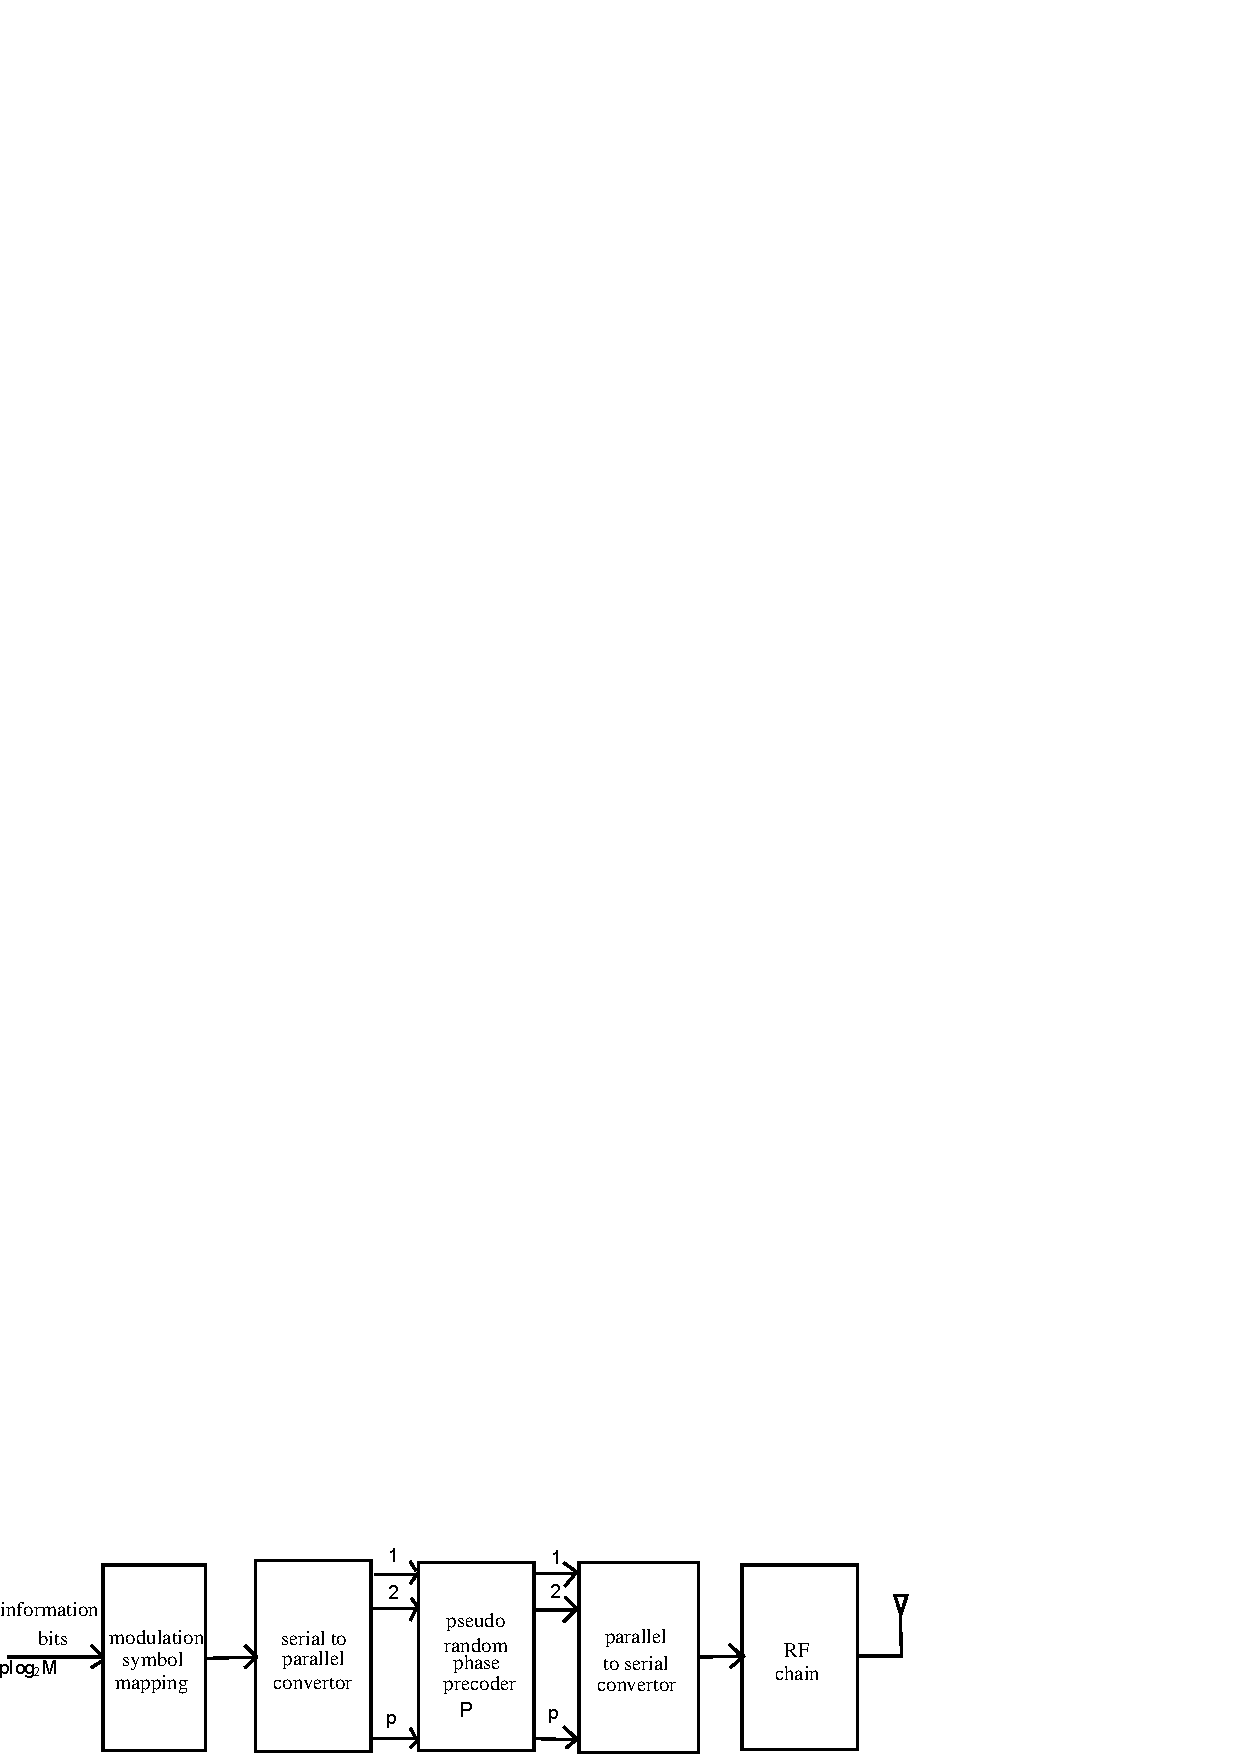
\includegraphics[scale=1]{sisoprecod.pdf}
\caption{PRPP transmitter.}
\label{prppblock}
%\end{center}
\end{figure}

\begin{eqnarray}
\vy_p&=& 
 \begin{bmatrix} 
   h_{(1)} & { 0} & \cdots & { 0} \\
   { 0}   & h_{(2)} & \cdots & { 0} \\
   \vdots & & \ddots & \vdots \\
   { 0} & { 0} & \cdots & h_{(p)}
 \end{bmatrix}\pp\mathbf s+\vn_p \nonumber\\
 &=&\md\pp\mathbf s + \vn_p=\mg\mathbf s + \vn_p,
\end{eqnarray}
where $\md=diag(h_{(1)}\, h_{(2)}\, \cdots\, h_{(p)})$, 
$\mg=\md\pp$, and $\vn_p$ is the noise vector 
$[\vn_{(1)}^T\, \vn_{(2)}^T\, \cdots\, \vn_{(p)}^T]^T$. The entries of the matrix $\mg$ are uncorrelated and 
$\lVert \md\rVert_F=\lVert \mg \rVert_F$. This creates a $p\times p$ 
virtual large-MIMO system.

The performance of PRPP transmission in a SISO system with MMSE-LAS detection algorithm [1], [2] is shown in Fig. \ref{sisoprecod}. It compares the average BER performance of the system without PRPP using ML detection against the performance of  PRPP transmission with MMSE-LAS detection. In Fig. \ref{sisoprecod}, we set the precoder size $p\in\{50,400\}$. It is interesting to note that the performance of MMSE-LAS detector approaches close to the AWGN system's performance when $p$ gets large.

\begin{figure}[htb]
\centering

\includegraphics[totalheight=9cm,width=12cm]{rameshfig.eps}
\caption{Performance of PRPP on SISO fading channels.}
\label{sisoprecod}
%\end{center}
\end{figure}


\section{Spatial modulation}
 Spatial modulation (SM) is a transmission scheme that uses multiple transmit antennas but only one transmit RF chain [3], [4]. At each time instant, only one among all the transmit antennas will be active and the others remain silent. The index of the active transmit antenna will also convey information bits in addition to the information bits conveyed through modulation symbols (e.g., QAM). The SM transmitter is shown in Fig. \ref{smtrans}, where the transmitter has $N_t$ transmit antennas but 
only one transmit RF chain. In a given channel use, 
the transmitter selects one of its $N_t$ transmit antennas, and transmits 
a modulation symbol from the modulation alphabet ${\mathbb A}$ on the selected antenna. 
The number of bits transmitted per channel use in the modulation symbols is 
$\lfloor \log_2|{\mathbb A}| \rfloor$, and the number of bits transmitted 
per channel use by the index of the transmitting antenna is 
$\lfloor \log_2N_t \rfloor$. Therefore, a total of 
$\lfloor \log_2|{\mathbb A}| N_t \rfloor$ bits per channel use (bpcu) is 
achievable in an SM-MIMO system. For example, in a system with $N_t=2$, and
8-QAM, the system throughput is 4 bpcu. 

\begin{figure}[htb]
\centering

\includegraphics[scale=1]{smtransmit.pdf}
\caption{SM transmitter.}
\label{smtrans}
%\end{center}
\end{figure}

The SM alphabet set for a fixed $N_t$ and $\sa$ is given by 
\begin{eqnarray}
\sm = 
\big \{ {\bf x}_{j,l}:j=1,\cdots,N_t, \ \ l=1,\cdots,|{\mathbb A}| \big \}, \nonumber \\ 
\mbox{s.t.} \ \ {\bf x}_{j,l} = 
[0,\cdots,0,\hspace{-4mm}\underbrace{s_{l}}_{{\scriptsize{\mbox{$j$th coordinate}}}}\hspace{-3.5mm},0,\cdots,0]^T, \ \ x_l \in \mathbb{A}.  
\end{eqnarray}
For example, for $N_t=2$ and 4-QAM, ${\mathbb S}_{N_t,{\mathbb A}}$ is given by  
{\small
\begin{eqnarray}
\hspace{-4mm}
{\mathbb S}_{2,\mbox{{\tiny 4-QAM}}}  
\hspace{-3mm}&=&\hspace{-3mm}\Bigg\{ 
\begin{bmatrix} +1+j \\ 0 \end{bmatrix}, 
\begin{bmatrix} +1-j \\ 0 \end{bmatrix}, 
\begin{bmatrix} -1+j \\ 0 \end{bmatrix}, 
\begin{bmatrix} -1-j \\ 0 \end{bmatrix}, \nonumber \\ 
& & 
\begin{bmatrix} 0 \\ +1+j \end{bmatrix}, 
\begin{bmatrix} 0 \\ +1-j \end{bmatrix}, 
\begin{bmatrix} 0 \\ -1+j \end{bmatrix}, 
\begin{bmatrix} 0 \\ -1-j \end{bmatrix} 
\Bigg \}. 
\end{eqnarray}
}

\vspace{-4mm}
Let $\vx \in {\mathbb S}_{N_t,{\mathbb A}}$ denote the transmit vector.
Let $\mh \in \mathbb{C}^{N_r\times N_t}$ denote the channel gain matrix,
where $H_{i,j}$ denotes the channel gain from the $j$th transmit antenna 
to the $i$th receive antenna and these channel gains are i.i.d complex 
Gaussian random variables. The received signal at the $i$th receive 
antenna is given by
\begin{equation}
y_i = H_{i,j}x_l + n_i,
\end{equation}
where $x_l$ is the $l$th symbol in ${\mathbb A}$, transmitted by the 
$j$th antenna, and $n_i$ is the noise which is distributed as
${\mathbb C}{\mathcal N}(0,\sigma^2)$. The signal at the receiver
can be written in vector form as
\begin{eqnarray}
\vy& = & \mh\vx+\vn,
\end{eqnarray}

For this system model, the maximum-likelihood (ML) detection rule is 
given by
\begin{equation} 
\label{ml1} 
\hat{\vx}=\argmin_{\vx\in \sm} \ \|\vy-\mh\vx\|^2,  
\end{equation}



In this work, we simultaneously exploit the advantages of both SM and PRPP. We propose a novel precoded SM scheme, where both the modulation bits and the antenna index bits are precoded using 
{\em pseudo-random phases}. We refer to this system as PRPP-SM system. The proposed PRPP-SM system gives significant performance improvement over SM system  without PRPP and PRPP system without SM. Since ML detection becomes exponentially complex in large dimensions, we propose a low complexity local search based detector (LSD) suited for PRPP-SM systems with large precoder 
sizes. Our simulation results show that  the proposed PRPP-SM achieves better performance than SM system without PRPP.
\chapter{Proposed PRPP-SM system}


In this work, we propose a novel precoded SM scheme, where
both the modulation bits and the antenna index bits are precoded by
pseudo-random phases. This gives an improvement in BER performance over SM system without PRPP. This improvement increases as the precoder size increases. As ML detection becomes exponentially complex in large 
dimensions, we propose a local search detector (LSD) which scales well for large precoder 
sizes. 

\section{System model}
The proposed PRPP-SM transmitter is shown in Fig. \ref{smprecod}.
First, $p$ modulated symbols are 
accumulated  to form the symbol vector $\vx_s \in \sa^p$, where $\mathbb A$ denotes the modulation alphabet. Let the matrix $\ma$ denote the antenna activation pattern, 
such that $\ma\vx_s \in \sm^p$, where $\sm$ denotes the SM alphabet set for a fixed $N_t$ and $\mathbb A$ is given by \begin{eqnarray}
\sm = 
\big \{ {\bf x}_{j,l}:j=1,\cdots,N_t, \ \ l=1,\cdots,|{\mathbb A}| \big \}, \nonumber \\ 
\mbox{s.t.} \ \ {\bf x}_{j,l} = 
[0,\cdots,0,\hspace{-4mm}\underbrace{s_{l}}_{{\scriptsize{\mbox{$j$th coordinate}}}}\hspace{-3.5mm},0,\cdots,0]^T, \ \ x_l \in \mathbb{A}.  
\end{eqnarray} The matrix $\ma$ consists of $p$ 
submatrices such that $\ma=[\ma_{(1)}^T \, \ma_{(2)}^T \, \cdots \, \ma_{(p)}^T]^T$, where $\mathbf A_{(i)}$ is the $i$th submatrix. The submatrix $\ma_{(i)}$ indicates the antenna activated in the
$i$th channel use. $\ma_{(i)}$ is a $N_t\times p$ matrix constructed as 
\begin{eqnarray}
\ma_{(i)}=[{\bf 0}_{(1)} \, \cdots \, {\bf 0}_{(i-1)} \, {\bf a}_{(i)} \, {\bf 0}_{(i+1)} \, \cdots \, {\bf 0}_{(p)}],
\end{eqnarray} 
where ${\bf 0}_{(k)}$ is a $N_t\times 1$ vector of zeroes, and 
${\bf a}_{(i)}$ is a $N_t\times 1$ vector constructed as
$[0 \, \cdots \, 0 \, \hspace{-2mm}\underbrace{1}_{\mbox{\tiny{$j_i$th coordinate}}} \hspace{-2mm} 0 \, \cdots \, 0]^T$, and $j_i$ is the index of the active antenna
during the $i$th channel use.

For example, in a system with $N_t=2$ and $p=3$, to activate antennas
1, 2 and 1 in three consecutive channel uses, respectively, the matrix 
$\ma$ is given by

\begin{figure}[t]
\centering

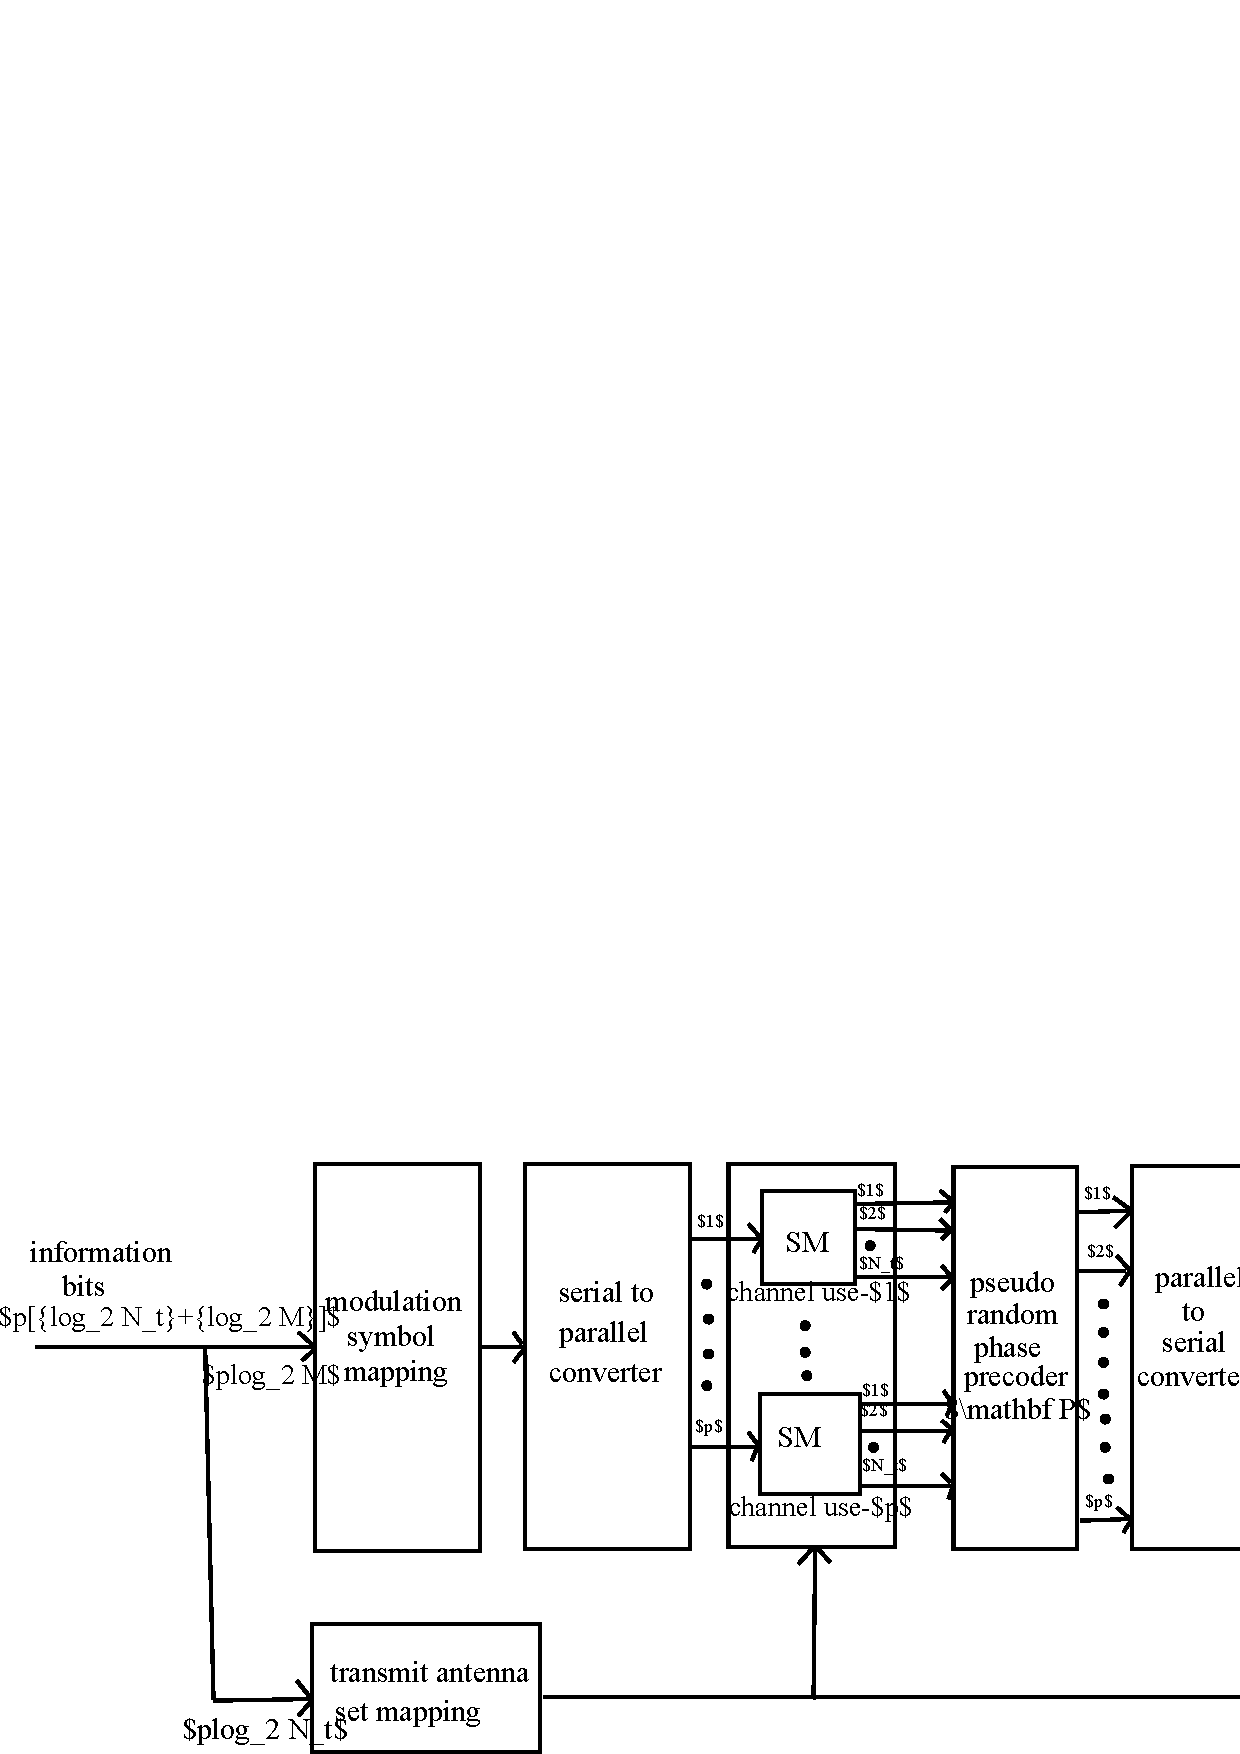
\includegraphics[scale=0.8]{rppsm.pdf}
\caption{Proposed PRPP-SM transmitter.}
\label{smprecod}
%\end{center}
\end{figure}

\begin{eqnarray}
\begin{bmatrix}
\ma_{(1)}\\
\ma_{(2)}\\
\ma_{(3)}
\end{bmatrix}&=&
 \begin{bmatrix}
1 & 0 & 0\\
0 & 0 & 0\\ \hdashline
0 & 0 & 0\\
0 & 1 & 0\\ \hdashline
0 & 0 & 1\\
0 & 0 & 0
 \end{bmatrix}
\end{eqnarray}

The matrix $\ma$ gives the support of the spatially modulated transmit
vector. The vector $\ma\vx_s \in \sm^p$ is precoded using a $p \times pN_t$ matrix $\pp$ to get $\pp\ma\vx_s$. 
The $(r,c)$th entry of the matrix $\pp$ is
$\frac{1}{\sqrt{p}}}e^{j\theta_{r,c}}$, where the phases 
$\theta_{r,c}$s are generated using a pseudo-random sequence generator. The seed of this generator is pre-shared among the transmitter and 
receiver. The output of the precoder is transmitted on the selected antenna in each channel use.
The signal received at the receiver after $p$ channel uses is given by
\begin{eqnarray}
\vy_p&=& 
 \begin{bmatrix} 
   \mh_{(1)} & {\bf 0} & \cdots & {\bf 0} \\
   {\bf 0}   & \mh_{(2)} & \cdots & {\bf 0} \\
   \vdots & & \ddots & \vdots \\
   {\bf 0} & {\bf 0} & \cdots & \mh_{(p)}
 \end{bmatrix}\ma\pp\ms\vx_s+\vn_p \nonumber\\
 &=&\md\ma\pp\ma\vx_s + \vn_p,
\end{eqnarray}
where $\md=diag(\mh_{(1)}\, \mh_{(2)}\, \cdots\, \mh_{(p)})$,  
 and $\vn_p$ is the noise vector 
$[\vn_{(1)}^T\, \vn_{(2)}^T\, \cdots\, \vn_{(p)}^T]^T$. For this system model, the ML detection rule is 
given by
\begin{equation} 
\label{ml3} 
\{\hat{\vx}_s,\hat{\ma}\}=\argmin_{\vx_s\in \sa^p, \forall \ma} \ \|\vy_p-\md\ma\pp\ma\vx_s\|^2,  
\end{equation}

The index of the non-zero row in each submatrix of  $\hat{\mathbf A}$ and values of $\hat{\mathbf x}_s$ are demapped to obtain the information bits.


\section{Proposed detection algorithm}

From (\ref{ml3}), it can be seen that the ML detection of the transmitted 
bits in a precoded SM-MIMO system is exponential in complexity, i.e.,
$O(|\sa|n_t)^p)$. We propose a local search based detector (LSD)
that achieves near-ML detection at large $p$ with a low computational 
complexity. The local search detector obtains a local minima in terms of
the least ML cost among a local neighborhood. The neighborhood is defined as follows. The set of neighbors of a given
pair of $\{\ma, \vx_s\}$, denoted by ${\mathcal N}(\ma, \vx_s)$, is defined as the 
set of all pairs $\{\ma', \vx_s'\}$ that satisfies one of the following 
three conditions:
\begin{enumerate}
\item
$\vx_s=\vx_s'$ and $\ma_{(i)}\neq\ma_{(i)}'$ for exactly a single index
$i$
\item 
$\ma=\ma'$ and $\vx_s$ differs from $\vx_s'$ in exactly one entry
\item
$\ma_{(i)}\neq\ma_{(i)}'$ for exactly a single index $i$, and for that 
index $i$, $x_s(i)\neq x'_s(i)$.
\end{enumerate}

For example, consider $N_t$=2, $p$=2, and  $\sa=\{\pm1\}$.  Then, we have
 


\vspace{0.5cm}
${\small
{\cal N}\left(\begin{bmatrix} 1&0 \\ 0&0 \\\hdashline 0&0 \\0&1\end{bmatrix},\begin{bmatrix} +1 \\ -1\end{bmatrix}\right)
\hspace{-1mm}=\hspace{-1mm}\left\{\begin{matrix}\vspace{0.5cm}
\{\begin{bmatrix} 1&0 \\ 0&0 \\\hdashline 0&1 \\0&0\end{bmatrix},\begin{bmatrix} +1 \\ -1\end{bmatrix}\},
\{\begin{bmatrix} 1&0 \\ 0&0 \\\hdashline 0&1 \\0&0\end{bmatrix},\begin{bmatrix} +1 \\ +1\end{bmatrix}\},
\{\begin{bmatrix} 1&0 \\ 0&0 \\\hdashline 0&1 \\0&0\end{bmatrix},\begin{bmatrix} -1 \\ -1\end{bmatrix}\},
\{\begin{bmatrix} 1&0 \\ 0&0 \\\hdashline 0&0 \\0&1\end{bmatrix},\begin{bmatrix} -1 \\ -1\end{bmatrix}\}\\

\vspace{0.5cm}


 \{\begin{bmatrix} 1&0 \\ 0&0 \\\hdashline 0&0 \\0&1\end{bmatrix},\begin{bmatrix} +1 \\ +1\end{bmatrix}\},
\{\begin{bmatrix} 0&0 \\ 1&0 \\\hdashline 0&0 \\0&1\end{bmatrix},\begin{bmatrix} +1 \\ -1\end{bmatrix}\},
\{\begin{bmatrix} 0&0 \\ 1&0 \\\hdashline 0&0 \\0&1\end{bmatrix},\begin{bmatrix} +1 \\ +1\end{bmatrix}\},
\{\begin{bmatrix} 0&0 \\ 1&0 \\\hdashline 0&0 \\0&1\end{bmatrix},\begin{bmatrix} -1 \\ -1\end{bmatrix}\}\end{matrix}
\right\}.
}$

The proposed LSD algorithm starts with an intial solution $\{\ma^{(0)}, \vx_s^{(0)}\}$, 
which is also the current solution. Using the defined neighborhood, the 
algorithm considers all the neighbors of $\{\ma^{(0)}, \vx_s^{(0)}\}$ and searches 
for the neighbor with the least ML cost which also has a lower ML cost 
than the current solution. If such a neighbor is found, then this neighbor 
is designated as the current solution. This marks the completion of one 
iteration of LSD. The iterations are repeated till a local minima is 
reached (i.e., there is no neighbor better than the current solution).  
The solution corresponding to the local minima is declared as the final 
output $\{\hat{\ma}, \hat{\vx}_s\}$. This algorithm is listed in 
{\bf Algorithm \ref{algo}}.

\begin{algorithm}[t]      
\caption{Listing of the proposed LSD}
   \begin{algorithmic} [1] 
      \STATE $\mathbf{Input: y, H}$,$\mathbf P$      
      \STATE Intial solution : $\{\ma^{(0)}, \vx_s^{(0)}\}$,  $\{\hat{\ma}, \hat{\vx}_s\}=\{\ma^{(0)}, \vx_s^{(0)}\}$
      \STATE Compute ${\cal N}(\hat{\ma}, \hat{\vx}_s)$
      \STATE $\{\ma^c, \vx_s^c\}$ = $\argmin\limits_{\{\mb,\vz\}\in{\cal N}(\hat{\ma}, \hat{\vx}_s)} \, \|\vy_p-\md\mb\pp\mb\vz\|^2$
	\IF{ $\|\vy_p-\md\ma^c\pp\ma^c\vx_s^c\|^2 < \|\vy_p-\md\hat{\ma}\pp\hat{\ma}\hat{\vx}_s\|^2 $}
	\STATE  $\{\hat{\ma}, \hat{\vx}_s\}=\{\ma^c, \vx_s^c\}$
	\STATE  Go to step 3
	\ENDIF 
      \STATE $\mathbf{Output}$ : $ \{\mathbf {\hat{A}},\mathbf {\hat{s}}\}$
\vspace{3mm}
\end{algorithmic}
\label{algo}
\end{algorithm} 

{\em Computing the intial solution}: We use MMSE for estimating the support and to 
obtain the initial solution to the LSD algorithm.  The MMSE
estimate is a $pN_t\times 1$ vector given by
$\vv=(\md^H\md+\sigma^2\mi)^{-1}\md^H\vy_p$. The vector $\vv$
consists of $p$ subvectors of size $N_t\times 1$,
$\vv=[\vv_{(1)}^T \,\vv_{(2)}^T \, \cdots \, \vv_{(p)}^T]^T$.
The indices of the elements with the largest amplitude in each
$\vv_{(i)}$ gives the initial solution for $\ma^{(0)}$. The  MMSE estimate of  $\vx_s ^{(0)}$ is given by a $p\times 1$ vector given by
$\vz=(\mg^H\mg+\sigma^2\mi)^{-1}\mg^H\vy_p$, where $\mathbf G=\mathbf H\mathbf \ma^{(0)}\mathbf P\mathbf \ma^{(0)} $. The hard estimate of $\vx_s^{(0)} $  is obtained by mapping each coordinate of $\vz$ to nearest symbol in the alphabet in terms of Euclidean distance.

\section{Simulation results}

We present the simulation results on the performance of the proposed PRPP-SM system with ML detection and MMSE-LSD. In all our simulations,  the channel is assumed to undergo temporally uncorrelated Rayleigh fading and independent between channel uses. 

Figure \ref{smml} compares the performance of PRPP-SM against the performance of SM without PRPP at a spectral efficiency of 3 bpcu using ML detection. Here, $N_t=4, N_r=1$ and BPSK modulation is used with precoder size  $ p \in\{2,4,5\}$. It is interesting to note that the performance of PRPP-SM is better than SM without PRPP by about 9 dB at $p=5$ and $10^{-2}$ BER. The performance of PRPP-SM gets even  better as $p$ increases.

Figure \ref{sisoml} compares the performance of PRPP-SM against the performance of PRPP without SM (i.e. $N_t=1$) at a spectral efficiency 3 bpcu using ML detection. Here, the PRPP-SM system has $N_t=4, N_r=1$, BPSK modulation, and PRPP system without SM  has $N_t=1, N_r=1$, 8-QAM  with precoder size  $ p \in\{2,4,5\}$. It is noted that the performance of PRPP-SM is better than the PRPP without SM by about 4 dB at $p=5$ and $10^{-2}$ BER. 

Figure \ref{smmmselas} compares the performance of PRPP-SM using MMSE-LSD detection against the performance of SM without PRPP using MLD at a spectral efficiency of 2 bpcu. Here PRPP-SM with $N_t=2, N_r=4$, and BPSK modulation is used with precoder size  $ p \in\{10,20,70\}$. It is seen that for smaller precoder sizes, PRPP-SM  performs poorer than SM without PRPP. But as the  precoder size increases, PRPP-SM performs better than SM without PRPP. At $10^{-5}$ BER, PRPP-SM with $p=70$ using MMSE-LSD detection is 1 dB  better than SM without PRPP using ML detection. This performance advantage in favor of PRPP-SM is expected to be even better for large values of $p$.

Figure \ref{sisolas} compares the performance of PRPP-SM using MMSE-LSD detection against the performance of PRPP without SM using MMSE-LAS detection, at a spectral efficiency 3 bpcu. For PRPP-SM we have used $N_t=4, N_r=8$, BPSK modulation. For PRPP without SM  we have used $N_t=1, N_r=8,$ 8-QAM.  The precoder size  $ p \in\{10,20,70\}$ in both systems. The spectral efficiency in both systems is 3 bpcu. It is observed that the performance of  PRPP-SM system is better than the PRPP system without SM by about 10 dB at $p$ = 70 and $10^{-2}$ BER. 






\begin{figure}[htb]
\centering

\includegraphics[totalheight=9cm,width=12cm]{prpp_sm_vs_withoutsm_ml.eps}
\caption{Performance comparison between PRPP-SM system $(N_t=4, N_r=1$, BPSK) with ML detection  and SM system without PRPP with ML detection. 3 bpcu.}
\label{smml}
%\end{center}
\end{figure}

\begin{figure}[htb]
\centering

\includegraphics[totalheight=9cm,width=12cm]{prppsiso_vs_sm_ml.eps}
\caption{Performance comparison between PRPP-SM system $(N_t=4, N_r=1$, BPSK) with ML detection  and  PRPP without SM $(N_t=1, N_r=1$, 8-QAM) with ML detection. 3 bpcu.}
\label{sisoml}
%\end{center}
\end{figure}

\begin{figure}[htb]
\centering

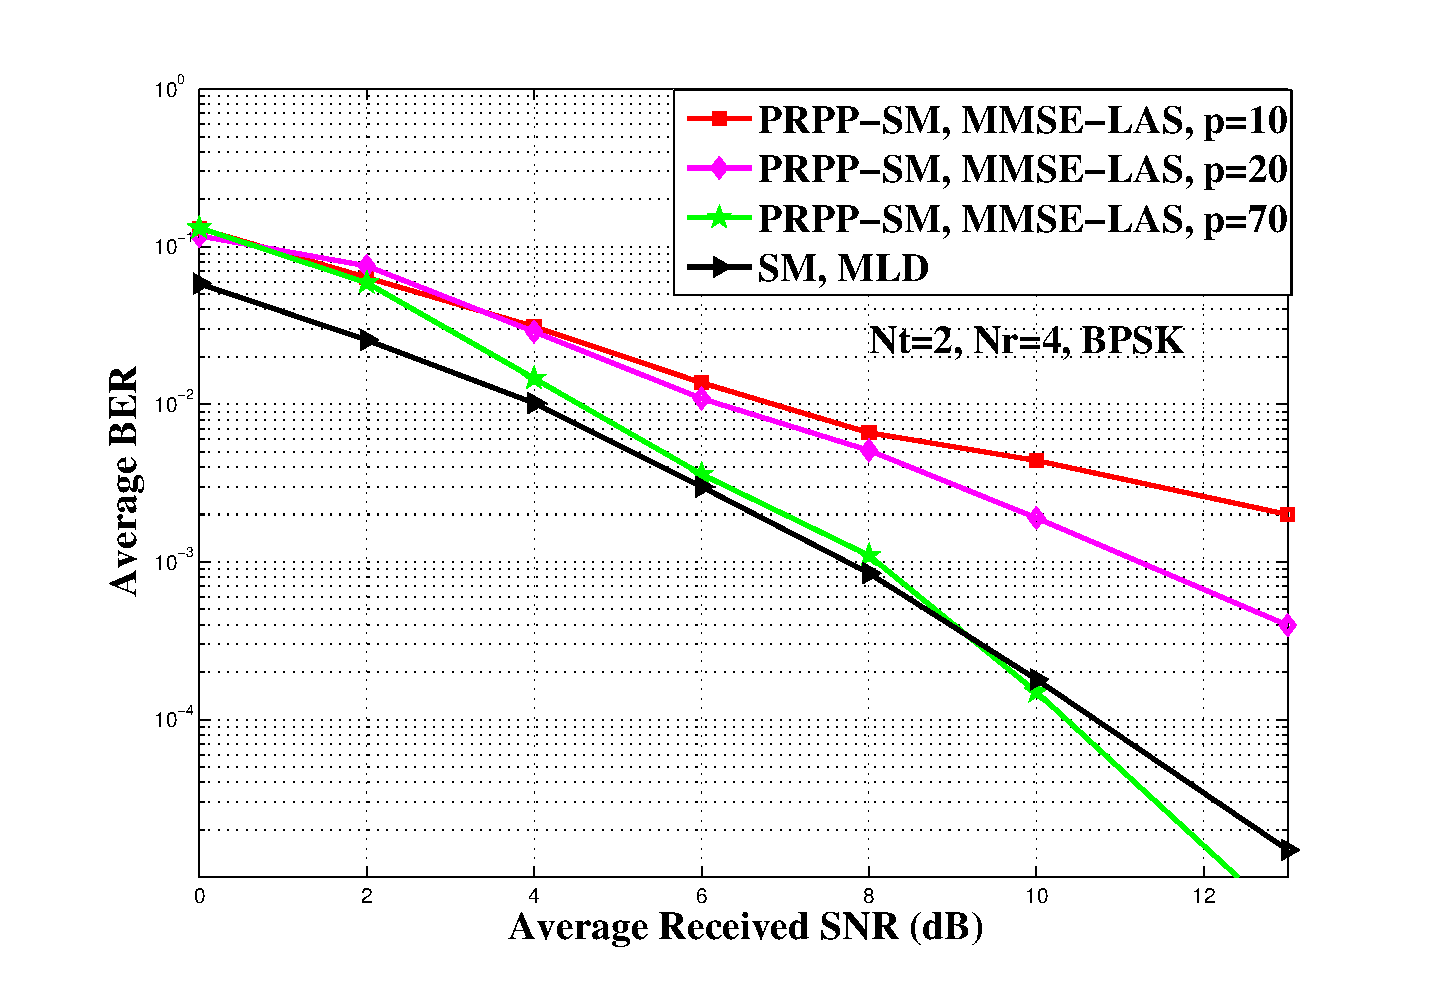
\includegraphics[totalheight=9cm,width=12cm]{prpp_sm_vs_withoutsm_mmse_las.eps}
\caption{Performance comparison between PRPP-SM $(N_t=2, N_r=4,$ BPSK) with LSD detection  and SM system without PRPP using ML detection. 2 bpcu.}
\label{smmmselas}
%\end{center}
\end{figure}
\begin{figure}[htb]
\centering

\includegraphics[totalheight=9cm,width=12cm]{prpp_sm_las.eps}
\caption{Performance comparison between PRPP-SM system $(N_t=4, N_r=8$, BPSK) with LSD detection  and PRPP without SM $(N_t=1,N_r=8$, 8-QAM) with LSD detection. 3 bpcu.}
\label{sisolas}
%\end{center}
\end{figure}


   
   \chapter{Conclusions and future work}
   
   We proposed a novel pseudo-random phase precoder based spatial modulation (PRPP-SM)  schemefor uncoded transmissions over fading channels. We assumed channel fades are independent and identically distributed across channel uses. With $N_t=4,N_r=1$, BPSK modulation, and ML detection, we demonstrated that the proposed PRPP-SM system achieves better performance than SM system without precoding and PRPP system without SM. We also proposed low complexity local search algorithm for detection in PRPP-SM systems  with large precoder sizes.
   With $N_t=4, N_r=1$, BPSK modulation, $5\times20$ precoder matrix and ML detection, we demonstrated that the proposed PRPP-SM system achieves better performance than the SM system without PRPP with ML detection by about 9 dB at $10^{-2}$ BER. The proposed system achieves increased diversity as the precoder size increases. In future, we will investigate the effect of time correlation on the performance of the PRPP-SM system.
   
  

 \begin{thebibliography}{99}
\vspace{0mm}

\bibitem{ic1}
R. Annavajjala and P. V. Orlik, ``Achieving near exponential diversity on uncoded low-dimensional MIMO, multi-user and multi-carrier systems without transmitter CSI, '' \textit{ Proc. ITA'2011}, Jan. 2011.
\bibitem{ic2} 
 K. V. Vardhan, S. K. Mohammed, A. Chockalingam, and B. S. Rajan,
``A low-complexity detector for large MIMO systems and multicarrier
CDMA systems,``\textit{ IEEE Journal on Selected Areas in Comm.}, vol. 26,
no. 3, pp. 473-485, Apr. 2008.

\bibitem{ic3} 
 R. Mesleh, H. Hass, S. Sinaovic, C. W. Ahn, ``Spatial modulation,''\textit{IEEE Trans.Veh.Tech.}, vol. 57, no. 4, pp. 2228-2241, Jul. 2008.
 
\bibitem{ic4}
 M. Di Renzo, H. Haas, A. Ghrayeb, S. Sugiura, and L. Hanzo, ``Spatial
modulation for generalized MIMO: challenges, opportunities and 
implementation,'' {\em Proceedings of the IEEE}, vol. 102, no. 1, pp. 53-55, Jan. 2014. 




\end{thebibliography}      
      



\end{document}